% Histogram of per-run mean score bucketed into 5 bins, one bar group per agent.
% Data derived from reports/eval_scores_v2_long.csv (mean of 4 evaluator composite scores per run).
% Buckets: [0,1), [1,2), [2,3), [3,4), [4,5]
\begin{figure}[t]
\centering
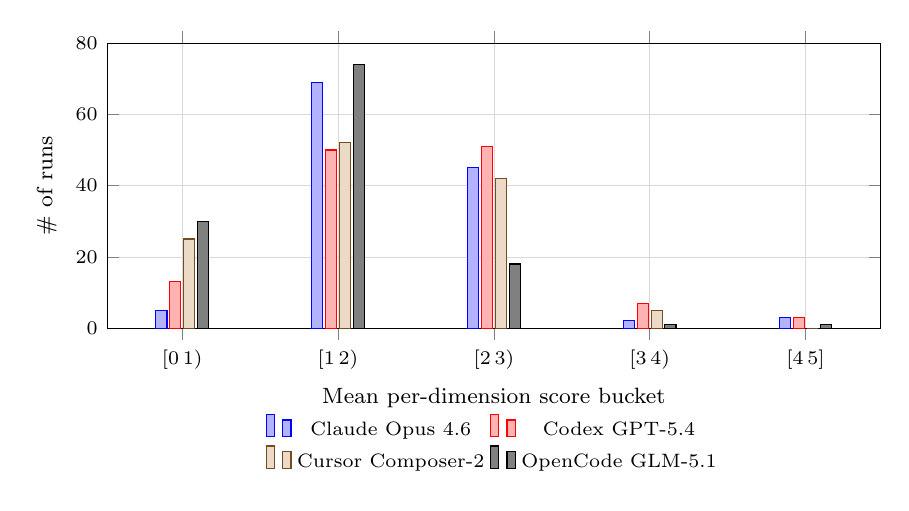
\begin{tikzpicture}
\begin{axis}[
  width=0.94\linewidth,
  height=5.2cm,
  ybar=1pt,
  bar width=4pt,
  symbolic x coords={[0\,1),[1\,2),[2\,3),[3\,4),[4\,5]},
  xtick=data,
  xlabel={\footnotesize Mean per-dimension score bucket},
  ylabel={\footnotesize \# of runs},
  ymin=0, ymax=80,
  enlarge x limits=0.12,
  legend style={font=\scriptsize, at={(0.5,-0.28)}, anchor=north, draw=none, legend columns=2},
  tick label style={font=\scriptsize},
  label style={font=\scriptsize},
  grid=both,
  major grid style={line width=0.2pt, draw=gray!30},
  minor tick num=0,
]
\addplot coordinates {([0\,1),5) ([1\,2),69) ([2\,3),45) ([3\,4),2) ([4\,5],3)};
\addplot coordinates {([0\,1),13) ([1\,2),50) ([2\,3),51) ([3\,4),7) ([4\,5],3)};
\addplot coordinates {([0\,1),25) ([1\,2),52) ([2\,3),42) ([3\,4),5) ([4\,5],0)};
\addplot coordinates {([0\,1),30) ([1\,2),74) ([2\,3),18) ([3\,4),1) ([4\,5],1)};
\legend{Claude Opus 4.6, Codex GPT-5.4, Cursor Composer-2, OpenCode GLM-5.1}
\end{axis}
\end{tikzpicture}
\caption{Per-run score distribution across four agents ($n{=}124$ runs each, combining 100 main-corpus and 24 calibration runs). Each bucket uses the mean per-dimension score, i.e., $(A+B+C)/3$ averaged across the four judges on a 0--5 scale; Table~\ref{tab:config-pass} reports the corresponding summed 0--15 composite mean. Most runs cluster in the 1--3 range, reflecting partial-pass behavior; full-rubric SE-PASS requires scores well above 4.}
\label{fig:score-histogram}
\end{figure}
